\documentclass{article}
% preamble v3.6

% v3.4
% - allowed tcolor theorem to break across columns and pages
% - updated tcolorbox theorem style

% v3.5
% - added more colors via xcolor

% v3.6
% - updated lstlisting style

% Layout packages
\usepackage{geometry}
\geometry{a4paper, margin=0.4in, top=0.7in}
\usepackage{multicol} % double column pages or more
\setlength\columnsep{20pt} % the default columnsep for all pages
\usepackage[none]{hyphenat} % no line breaking on words
\usepackage{parskip} % typical paragraphs - no indent, vertical space between paragrahs
\usepackage{titlesec} % reduced vertical space around section titles

% Alter typesetting of headers and footers
\usepackage{fancyhdr}
\pagestyle{fancy}
\fancyhf{}
\fancyhead[L]{\textbf{CS2102 --- Database Systems}}
\fancyhead[R]{\textbf{\thepage}}
\setlength{\headheight}{2em}
\renewcommand{\headrulewidth}{2pt}

% Math packages
% https://tex.stackexchange.com/questions/32100/what-does-each-ams-package-do
\usepackage{amssymb}
\usepackage[fleqn]{amsmath}
% \usepackage{cancel} % cancelling symbols - unused
% \usepackage{bm} % bold and italicize math - unused
\usepackage{siunitx} % SI units with \si{...}

% Font packages
\usepackage[utf8]{inputenc}
\usepackage{arev}
\usepackage[sfdefault]{inter}
\usepackage[T1]{fontenc}
\usepackage{microtype}

% Color packages
\usepackage[dvipsnames]{xcolor} % custom named colors
\definecolor{body}{HTML}{555555}
\definecolor{background}{HTML}{FFFFFF}
\definecolor{m_purple}{HTML}{C39AC9}
\definecolor{m_blue}{HTML}{9CD1BB}
\definecolor{m_red}{HTML}{FF657A}
\definecolor{m_green}{HTML}{BAD761}

% Image & graphics packages
% \usepackage{graphicx} - unused (no graphics)
% \graphicspath{ {./images/} }
% \usepackage[linguistics]{forest} % unused (no trees)

% Better enumerate/itemize environment
\usepackage{enumerate}
\usepackage{enumitem} % all list modifications - remove enumerate spacing with [leftmargin=*]
\setlist{nolistsep} % remove spacing in and around lists
\setlist[itemize]{leftmargin=*, itemsep=0.15em} % remove natural first level indent and customize spacing
\setlist[enumerate]{leftmargin=*, itemsep=0.15em} % remove natural first level indent and customize spacing
\renewcommand{\labelitemi}{\textsc{--}} % change first level bullet to --
\renewcommand{\labelenumii}{\theenumii} % change enumerate numbering to arabic
\renewcommand{\theenumii}{\theenumi.\arabic{enumii}.}
\renewcommand{\labelenumiii}{\theenumiii}
\renewcommand{\theenumiii}{\theenumii\arabic{enumiii}.}

% Better table environments
\usepackage{tabularx} % deprecated - use tabularrray instead - fit columns to width with \tabularx{\linewidth}{X}
\renewcommand{\arraystretch}{1.25}
\usepackage{arydshln} % dashed lines in tables
\newcolumntype{Y}{>{\centering\arraybackslash}X} % centered tabularx X columns with Y
\usepackage{tabularray} % modern table typesetting, superseding tabularx
\usepackage{multirow} % row merging in tables
\NewColumnType{Y}[1][c]{Q[#1, \linewidth]}

% Better code environments
\usepackage{listings}
\newcommand{\code}[1]{\texttt{#1}}

% Custom typesetting values
\setlength{\abovedisplayskip}{0pt}
\setlength{\belowdisplayskip}{0pt}
\setlength{\abovedisplayshortskip}{0pt}
\setlength{\belowdisplayshortskip}{0pt}
\setlength{\mathindent}{0pt} % no indent for all math (including the align) environemnts

% Custom commands
\newcommand{\pageline}[1]{\par\noindent\rule{\textwidth}{#1}} % horizontal lines across a page
\newcommand{\quoted}[1]{\textquotedblleft{#1}\textquotedblright} % proper double quotes
\NewDocumentCommand{\keyitem}{smm}{\item \textbf{#2}: \IfBooleanF{#1}{\\ }#3} % bolded keywords in list environments, use * for no newline separation

% Custom environments
\newenvironment{itemize*}{\begin{itemize}[itemsep=0.5em]}{\end{itemize}}
\newenvironment{enumerate*}{\begin{enumerate}[itemsep=0.5em]}{\end{enumerate}}
\renewenvironment{boxed}[1][c]{\begin{tblr}{hlines, vlines, colspec={Y[#1]}}}{\end{tblr}}

% https://tex.stackexchange.com/questions/247185/tcolorbox-theorem-which-isnt-framed-on-the-sides
\usepackage{tcolorbox}
\tcbuselibrary{theorems}
\tcbuselibrary{skins}
\tcbuselibrary{breakable}
\newtcbtheorem[]{thm}{}{
    breakable,
    theorem style=change apart,
    description delimiters none,
    enhanced,
    frame hidden,
    % interior hidden,
    boxrule=0pt,
    left=0.2cm,right=0.2cm,
    toptitle=0.1cm+2pt,
    bottomtitle=-0.05cm+0.5em,
    colframe=body,colback=white,coltitle=white,
    title style=body,
    bottomrule=1pt,
    borderline south={1pt}{0pt}{body},
    fonttitle=\bfseries,fontupper=\normalsize
}{thm}
\newenvironment{defn}[1]{
    \begin{thm*}{#1}\color{body}
    \setlength{\abovedisplayskip}{0pt}
    \setlength{\belowdisplayskip}{0.75em}
    \setlength{\abovedisplayshortskip}{0pt}
    \setlength{\belowdisplayshortskip}{0.75em}
    \setlength{\parskip}{0.5em}
    \vspace{-\parskip}
}{\end{thm*}}
\newenvironment{defn*}[1]{
    \begin{thm*}{#1}\color{body}
    \setlength{\abovedisplayskip}{0pt}
    \setlength{\belowdisplayskip}{0.75em}
    \setlength{\abovedisplayshortskip}{0pt}
    \setlength{\belowdisplayshortskip}{0.75em}
    \setlength{\parskip}{0.5em}
}{\end{thm*}}

% CS2102 specific
% functional dependencies
\newcommand{\fd}[2]{${#1} \rightarrow {#2}$}

% postgre keywords
\lstdefinelanguage{postgre}{%
  language     = SQL,
  morekeywords = {OFFSET},
}
\lstset{
  language=postgre,
  showstringspaces=false,
  columns=flexible,
  aboveskip=1.5em,
  belowskip=0.5em,
  frame=bt,
  numbers=none,
  basicstyle={\linespread{1.5}\small\ttfamily},
  commentstyle={\color{body!60}\textit},
  breaklines=true,
  breakatwhitespace=true,
  tabsize=4
}

% outer join symbols
% https://tex.stackexchange.com/questions/20740/symbols-for-outer-joins
\def\ojoin{\setbox0=\hbox{$\bowtie$}%
  \rule[-.02ex]{.25em}{.4pt}\llap{\rule[\ht0]{.25em}{.4pt}}}
\def\leftouterjoin{\mathbin{\ojoin\mkern-5.8mu\bowtie}}
\def\rightouterjoin{\mathbin{\bowtie\mkern-5.8mu\ojoin}}
\def\fullouterjoin{\mathbin{\ojoin\mkern-5.8mu\bowtie\mkern-5.8mu\ojoin}}

% ER diagrams
\usepackage{tikz}
\usetikzlibrary{er,positioning,arrows.meta}

\color{body}
\pagecolor{background}
\frenchspacing

\title{\vspace{-1cm}\textbf{CS2102 \\[0.25em] Database Systems} \\[2em] \Large AY2022/23 Semester 2 \\[1em]}
\author{Notes by Jonathan Tay}
\date{Last updated on \today}

\begin{document}
\linespread{1.4}\selectfont
\pagenumbering{gobble} % remove page numbering for content pages
\maketitle
\pageline{1.5pt}
\tableofcontents
\pageline{1.5pt}
\linespread{1.1}\selectfont

\newpage
\pagenumbering{arabic} % re-add page numbering
\begin{multicols*}{2}
    \part{Relational and ER Models}
    \part{Relational Model}

Data in \textbf{relational databases} are stored in \textbf{relations} (tables).
Column headers are \textbf{attributes}, and rows are \textbf{tuples}.

The \textbf{degree} is the number of columns, and the \textbf{cardinality} is the number of rows.

The \textbf{domain} of an attribute $A_i$, denoted as $\operatorname*{dom}(A_i)$,
is the set of all possible \textit{atomic} values for $A_i$.
\code{NULL} is an additional special value for unknown or invalid values.


\begin{defn}{keys}
    A \textbf{superkey} is a subset of attributes that uniquely identifies a tuple.
    A \textbf{key} is a \textit{minimal} superkey.

    The \textbf{candidate keys} is the set of all keys for a relation, of which
    one is selected as a \textbf{primary key}.

    Primary key values must be non-\code{NULL}.
\end{defn}

\begin{defn}{foreign keys}
    A \textbf{foreign key} is a subset of attributes of a \textit{referencing relation}
    that refers to the primary key of a \textit{referenced relation}:

    (referencing attributes) $\rightsquigarrow$ (referenced attributes)

    Because the names of the attributes are not necessarily unique,
    each attribute is prefixed with the name of the relation, like so:

    (<relation name> $\cdot$ <attribute name>, ...) $\rightsquigarrow$ ...

    Foreign keys must appear as a primary key in the referenced table,
    \code{NULL}, or a tuple containing \code{NULL}.
\end{defn}

The key constraints above are not intrisic properties of a relation; rather, they are specified by the database designer to avoid problematic but otherwise valid data.

\section{Relational Algebra}

Relation are always the \textbf{operands} in relational algebra, on which \textbf{operators} are applied.

Because relations are closed under \textit{any combination of operators}, the result of an operation is \textit{always} a relation, and no other output is possible (\textbf{closure property}).

\begin{defn}{3-valued logic (\code{false}, \code{true}, and \code{NULL})}
    Any operation involving \code{NULL} will result in \code{NULL}.
    Hence, $\equiv$ and $\not\equiv$ are needed to compare (in)equality of \code{NULL} values directly:

    \code{NULL} = \code{NULL} produces \code{NULL}, but \code{NULL} $\equiv$ \code{NULL} produces \code{true}.

    \begin{tblr}{
        colspec={XX||XXX},
        hlines, vlines,
        row{1,2} = {font=\bfseries},
        column{1,2} = {font=\bfseries},
        cell{1}{1} = {c=2,r=2}{c},
        cell{1}{3} = {c=3}{c},
        cell{3}{1} = {r=3}{c},
        cell{4}{2,3,4,5} = {m_red!20},
        cell{2,3,4,5}{4} = {m_red!20},
        cell{2,3}{3} = {m_green!20},
        cell{3}{2} = {m_green!20},
        cell{5}{2,3,5} = {m_blue!20},
        cell{2,3,5}{5} = {m_blue!20},
    }
        $a \land b$ & & $a$ \\
        & & \code{true} & \code{false} & \code{NULL} \\ \hline
        $b$ & \code{true} & \code{true} & \code{false} & \code{NULL} \\
        & \code{false} & \code{false} & \code{false} & \code{false} \\
        & \code{NULL} & \code{NULL} & \code{false} & \code{NULL}
    \end{tblr}

    \begin{tblr}{
        colspec={XX||XXX},
        hlines, vlines,
        row{1,2} = {font=\bfseries},
        column{1,2} = {font=\bfseries},
        cell{1}{1} = {c=2,r=2}{c},
        cell{1}{3} = {c=3}{c},
        cell{3}{1} = {r=3}{c},
        cell{2}{4} = {m_red!20},
        cell{4}{2,4} = {m_red!20},
        cell{3}{2,3,4,5} = {m_green!20},
        cell{2,3,4,5}{3} = {m_green!20},
        cell{5}{2,4,5} = {m_blue!20},
        cell{2,4,5}{5} = {m_blue!20},
    }
        $a \lor b$ & & $a$ \\
        & & \code{true} & \code{false} & \code{NULL} \\ \hline
        $b$ & \code{true} & \code{true} & \code{true} & \code{true} \\
        & \code{false} & \code{true} & \code{false} & \code{NULL} \\
        & \code{NULL} & \code{true} & \code{NULL} & \code{NULL}
    \end{tblr}
\end{defn}

\subsection{Equivalence and Compatibility}
Two \textit{expressions} are \textbf{equivalent} if either \textit{both} produce an error, or \textit{both} produce the same result.

Errors occur if attributes are missing (e.g. by projection or renaming), or
are incompatible --- there is no implicit type conversion.

The order of types in a tuple matters --- (\code{int}, \code{text}) is not equivalent to (\code{text}, \code{int}).

Two \textit{relations} are \textbf{union-compatible} if they have the same number of attributes with the same domain (type).

\subsection{Basic Operators}
Note that logical conjunction ($\land$) has greater precedence than logical disjunction ($\lor$).

\begin{defn}{selection --- $\sigma_{[c]}(R)$}
    Filters the rows of relation $R$, returning the set of tuples that satisfy the condition $c$.

    Conditions which evaluate to \code{NULL} are excluded from the result.

    The condition $c$ must only specify attributes of $R$.
\end{defn}

\begin{defn}{projection --- $\pi_{[l]}(R)$}
    Maps the relation $R$, returning the set of tuples with the attributes in the ordered list $l$, in the order specified by $l$.

    Equivalent to a column filter, but the rows which were previously unique tuples may no longer be unique, and are therefore de-duplicated.

    The elements of $l$ must not be operations, must be attributes of $R$, and must be unique.
\end{defn}

\begin{defn}{renaming --- $\rho_{[\mathcal{R} ]}(R)$}
    Renames the attributes of relation $R$ to the attributes in the unordered list $\mathcal{R}$.

    Elements of $\mathcal{R}$ must be in the following form: \\
    $\text{<new name>} \leftarrow \text{<old name>}$.

    New attribute names must be unique, and existing attributes must only be renamed at most once per operation (i.e. $\rho_{[A \leftarrow B, B \leftarrow C]}$ is invalid).
\end{defn}

\subsection{Set Operators}
The typical set union ($\cup$), set intersection ($\cap$), and set difference ($-$) operators are omitted for brevity.

\begin{defn}{cross product --- $R \times S$}
    For every tuple in $R$, concatenate it with every tuple in $S$ to form a new relation, such that the cardinality (number of rows) of the result is $|R| \times |S|$.

    The set of attributes in $R$ and $S$ must be disjoint, such that the degree (number of columns) of the result is $\operatorname*{deg}(R) + \operatorname*{deg}(S)$.

    Cross products are associative --- $R \times (S \times T) = (R \times S) \times T$.
\end{defn}

\subsection{Join Operators}
\textbf{Joins} are a composite operator, composing cross product, selection, and projection on a relation.

This concatenates two tables and removes unwanted/redundant rows and columns from the result of a cross product.

\begin{defn}{theta-join ($\theta$-join) --- $R \Join_{[\theta]} S$}
    Cross $R$ and $S$, then filter (by selection) the rows using the condition $\theta$.
\end{defn}

\begin{defn}{equi-join --- $R \Join_= S$}
    A special case of theta-join, where only equality ($=$) conditions are allowed (c.f. $\theta$-join which allows $\equiv$, $\le$, $<>$, etc.).

    This may be more performant versus a theta-join as hashing can be used internally.
\end{defn}

\begin{defn}{natural inner join --- $R \Join S$}
    First, find the set of attributes that are common to both $R$ and $S$.

    Then, cross $R$ and $S$, and retain (by selection) the rows for which the \textbf{common attributes} are equal --- this also eliminates rows with any \code{NULL} value.
    
    If there are no common attributes, then this is simply the cross product (by vacuous truth).

    Finally, de-duplicate (by projection) the columns by their attribute names.

\end{defn}

Theta-joins, equi-joins, and natural inner joins are collectively known as \textbf{inner joins}.

If we wish to perform a join but still retain \textit{all rows} from the \textit{left} table, \textit{right} table, or even \textit{both} tables and simply pad missing values with \code{NULL}, we can use \textbf{outer joins}.

\begin{defn}{full outer join --- $L \fullouterjoin_{[\theta]} R$}
    \begin{tblr}{
        colspec = {Xl|Xl},
        cell{1}{1,3} = {c=2}{l},
        row{2,3} = {m_red!20},
        row{4,5} = {m_green!20},
        row{6,7} = {m_blue!20}
      }
      \hline[2pt]
        \textbf{attributes of $L$} && \textbf{attributes of $R$} \\
      \hline[1pt]
            values from $L$ & $\cdots$ & values from $R$ & ... \\
            $\vdots$ & $\ddots$ & $\vdots$ & $\ddots$ \\
            values from $L$ & ... & \code{NULL} & ... \\
            $\vdots$ & $\ddots$ & $\vdots$ & $\ddots$ \\
            \code{NULL} & ... & values from $R$ & ... \\
            $\vdots$ & $\ddots$ & $\vdots$ & $\ddots$ \\
      \hline[2pt]
    \end{tblr}

    Inner joins only retain rows (in \textcolor{m_red}{red}) from which both $L$ and $R$ have a value for which the condition $\theta$ evaluates to \code{true} (during the selection).

    However, rows (in \textcolor{m_green}{green} and \textcolor{m_blue}{blue}) which do not satisfy $\theta$ may also be desirable, and can be retained by outer joins.

    The \textbf{full outer join} retains all of the rows above.
\end{defn}

\begin{defn}{left outer join --- $L \leftouterjoin_{[\theta]} R$}
    The left outer join retains the \textcolor{m_red}{red} and \textcolor{m_green}{green} rows.
\end{defn}

\begin{defn}{right outer join --- $L \rightouterjoin_{[\theta]} R$}
    The left outer join retains the \textcolor{m_red}{red} and \textcolor{m_blue}{blue} rows.
\end{defn}

\begin{defn}{natural outer joins}
    The natural keyword can be prefixed to the left, right, or full outer joins, e.g. "natural left outer join".

    The equality condition is implicitly defined over the set of attributes that are common to both $L$ and $R$.
\end{defn}
    \section{Entity Relationship Model}
In the ER model, data is described as a collection of:
\begin{itemize*}
    \keyitem{entities}{representation of real-world objects that are distinguishable from other objects}
    \keyitem{relationships}{associations between one or more entities}
\end{itemize*}

Entities and relationships of the same type form \textbf{entity sets} and \textbf{relationship sets} respectively.

\textbf{Attributes} describe information about entities and relationships, and there are various kinds:
\begin{itemize}
    \keyitem*{key}{uniquely identify an entity}
    \keyitem*{composite}{collection of multiple \textit{attributes}}
    \keyitem*{multivalued}{collection of multiple possible \textit{values}}
    \keyitem*{derived}{calculated from other attributes}
\end{itemize}

\vspace{1em}
\begin{tikzpicture}[
    auto,
    node distance=1cm,
    every entity/.style={fill=m_blue!20,draw=m_blue,thick},
    every attribute/.style={fill=m_green!20,draw=m_green,thick},
    every relationship/.style={fill=m_red!20,draw=m_red,thick,aspect=1.5}]
]
    \node[entity] (node1) {entity set}
    [grow=up,sibling distance=4cm]
    child[grow=up] {node[attribute] (composite) {composite attr.}}
    child[grow=left,level distance=2.5cm] {node[attribute] {\underline{key attr.}}};

    \node[attribute] (simple1) [above left = of composite] {attribute};
    \path (simple1) edge node {} (composite);
    \node[attribute] (simple2) [above = of composite] {attribute};
    \path (simple2) edge node {} (composite);
    \node[attribute] (simple3) [above right = of composite] {attribute};
    \path (simple3) edge node {} (composite);

    \node[relationship] (rel1) [below = of node1] {relationship};
    \node[entity] (node2) [above right = of rel1] {entity set}
    [grow=right,sibling distance=3cm]
    child {node[attribute, double] {multivalued}}
    child {node[attribute, dashed] {derived attr.}};

    \path (rel1) edge node {role label} (node1) edge node {} (node2);
\end{tikzpicture}
\vspace{1em}

The \textbf{degree} (or \textit{arity}) of a relationship set is the number of entity sets involved --- binary for $n = 2$, ternary for $n = 3$.

\subsection{Relationship Constraints}

\begin{defn}{cardinality constraints}
    Relationships can be \textbf{many-to-many}, \textbf{many-to-one}, or \textbf{one-to-one}. These are \textit{upper bounds}.

    The default upper limit is $\infty$, and setting an upper limit of $1$ is depicted in ER diagrams by an arrowhead:

    \vspace{0.5em}
    \begin{tikzpicture}[
        auto,
        node distance=1cm,
        every entity/.style={fill=m_blue!20,draw=m_blue,thick},
        every attribute/.style={fill=m_green!20,draw=m_green,thick},
        every relationship/.style={fill=m_red!20,draw=m_red,thick,aspect=1.5}]
    ]
        \node[entity] (E) {entity set};
        \node[relationship] (R) [right = of E] {relationship};
        \path[{Stealth[length=3mm, width=2mm]}-] (R) edge node {} (E);
    \end{tikzpicture}
\end{defn}

\begin{defn}{participation constraints}
    Participation constraints can be \textbf{partial} (0 or more) or \textbf{total} (1 or more). These are \textit{lower bounds}.

    The default lower limit is $0$, and setting a lower limit of $1$ is depicted in ER diagrams by a double line:

    \vspace{0.5em}
    \begin{tikzpicture}[
        auto,
        node distance=1cm,
        every entity/.style={fill=m_blue!20,draw=m_blue,thick},
        every attribute/.style={fill=m_green!20,draw=m_green,thick},
        every relationship/.style={fill=m_red!20,draw=m_red,thick,aspect=1.5}]
    ]
        \node[entity] (E) {entity set};
        \node[relationship] (R) [right = of E] {relationship};
        \path (R) edge[double distance = 1.5 pt, black] node {} (E);
    \end{tikzpicture}
\end{defn}

\begin{defn}{dependency constraint}
    A \textbf{weak entity set} does not have its own key, instead having a \textbf{partial key} which can only uniquely identify entities with a primary key from its \textbf{owner entity set}.

    This requires a connection via an \textbf{identifying relationship set}:

    \begin{tikzpicture}[
        auto,
        node distance=1cm,
        every entity/.style={fill=m_blue!20,draw=m_blue,thick},
        every attribute/.style={fill=m_green!20,draw=m_green,thick},
        every relationship/.style={fill=m_red!20,draw=m_red,thick,aspect=1.5}]
    ]
        \node[entity, double] (E) {weak entity set};
        \node[relationship] (R) [above right = of E] {relationship};
        \path[{Stealth[length=3mm, width=2mm]}-] (R) edge[double distance = 1.5 pt, black] node {} (E);
        \node[entity] (O) [right = of E] {owner entity set};
        \path (R) edge node {} (O);
    \end{tikzpicture}
\end{defn}
    \part{SQL}
\textbf{SQL} (Structured Query Language) is case-insensitive, but keywords are uppercase by convention.

The most common data types are \code{INTEGER}, \code{VARCHAR(n)}, \code{BOOLEAN}, and \code{DATE}.

\section{Operations and Syntax}

\subsection{Table Operations}
\begin{lstlisting}
CREATE TABLE table_name (
    -- define attributes (columns)
    <attribute> <type> [<column_constraint>],
    <attribute> <type> [CONSTRAINT <name> <cstr.>],
    ...
    -- define optional table constraints
    [<table_constraint>],
    -- constraints can be named
    [CONSTRAINT <name> <table_constraint>],
    ... /* alternative comment syntax */
    [<table_constraint>] -- no trailing comma
);

ALTER TABLE <table>
    [ALTER / ADD / DROP] [COLUMN / CONSTRAINT]
    <attribute / name>
    <changes>;

DROP TABLE
    [IF EXISTS] -- no error if table doesn't exist
    <table>, ... -- drop multiple tables at once
    [CASCADE]; -- also drop referencing tables
\end{lstlisting}

\subsection{Integrity Constraints}
Constraints are specified in the \code{CREATE TABLE} statement,
and reject insertions if the condition evaluates to \code{false} (\textbf{principle of rejection}).

\textbf{Column constraints} are defined on a per-column basis, while \textbf{table constraints} are defined on the table as a whole.

Constraints can be \textit{named}, or \textit{unnamed}, in which case the DBMS will generate a name.

There are 5 types of constraints that can be placed on a table $R$ and/or any attribute $a$:
\begin{enumerate*}
    \keyitem*{\code{NOT NULL}}{$\forall r \in R: r_a \not\equiv \code{NULL}$}
    \keyitem*{\code{UNIQUE}}{$\forall r_1, r_2 \in R: (r_1 \equiv r_2) \lor (\exists r_{1_a} <> r_{2_a})$}
    \keyitem*{\code{PRIMARY KEY}}{equivalent to \code{UNIQUE} and \code{NOT NULL}}
    \keyitem{\code{FOREIGN KEY ($a, ...$) REFERENCES $R'$($a', ...$)}}{$\forall r \in R: (\forall a: r_a \in R_{a'}') \lor (\code{NULL} \in r)$}
    \keyitem*{\code{CHECK($c$)}}{$c$ does not evaluate to \code{false}}
\end{enumerate*}

For \code{UNIQUE}, note that \code{NULL} $<>$ \code{NULL} evaluates to \code{NULL},
such that duplicate insertions of \code{NULL} are not rejected.

For \code{FOREIGN KEY}, $R'$ must be a valid table name. \\
\code{SET NULL}, \code{SET DEFAULT}, or \code{CASCADE} can be specified as the action to take when a referenced row is deleted.

\code{CASCADE} will delete all referencing rows, propagating the deletion, which may significantly affect performance.

For \code{CHECK}, $c$ must be a boolean expression scoped to the table on individual rows.

\subsection{Row Operations}
\begin{lstlisting}
INSERT INTO <table> [(attribute, ...)]
    VALUES -- whitespace and newlines optional
        (value, ...),
        (value, ...),
        ... -- alternatively, all on one line
        (value, ...);
\end{lstlisting}

All values to insert must have the same shape as either the table, or, if specified, the attribute list.

Attributes in the attribute list can be in any order.

Attributes missing from the attribute list will have their values set to \code{NULL}, or, if specified in the schema, to their default value.

\begin{lstlisting}
DELETE FROM <table> [WHERE <condition>];
\end{lstlisting}

The condition only deletes rows which evaluate to \code{TRUE} (\textbf{principle of acceptance}).

If the condition is omitted, all rows will be deleted.

The condition must be a boolean expression scoped to to the table on individual rows.

\subsection{Deferrable Constraints}
\begin{lstlisting}
BEGIN; -- start a transaction
-- perform operations
COMMIT; -- commit (end) the transaction
\end{lstlisting}

Constraints are checked immediately at the end of every SQL statement (these end with a semicolon) and transaction --- violation performs a rollback.

When defining a constraint, three deferments can be specified:
\begin{enumerate*}
    \keyitem{\code{NOT DEFERRABLE}}{if unspecified, this is the default}
    \keyitem{\code{DEFFERABLE INITIALLY IMMEDIATE}}{constraint is checked immediately, but can be deferred later}
    \keyitem{\code{DEFFERABLE INITIALLY DEFERRED}}{constraint is deferred by default}
\end{enumerate*}

\code{DEFFERABLE INITIALLY IMMEDIATE} gives the \textit{option} to defer the constraint checking by adding the following line in a transaction, i.e.:

\begin{lstlisting}
BEGIN;
SET CONSTRAINTS <name> DEFERRED; -- add this line
-- perform operations
COMMIT;
\end{lstlisting}

Deferring a constraint is necessary when the constraint depends on a row that is inserted later in the transaction, e.g. circular foreign key constraints.
    \part{Normal Forms}
A \textbf{normal form} is a definition of minimum requirements to reduce data redundancy and improve data integrity.

Redundancies can lead to \textbf{anomalies} where a primary key attribute violates the constraint of being non-\code{NULL}.

These anomalies can be resolved by \textbf{normalization}.


\section{Functional Dependencies}
A \textbf{functional dependency} is a relationship between two sets of attributes $A$ and $B$ that occur when the value of $B$ can always be determined from the value of $A$.

That is, when $A_1 A_2 \dots A_m \rightarrow B_1 B_2 \dots B_n$, any tuple with the same values for $A_1 A_2 \dots A_m$ will have the same value for $B_1 B_2 \dots B_n$.

\begin{defn}{determining functional dependencies}
    Intuitively, the $\rightarrow$ can be read as "decides" or "determines".

    Given attributes $A$ and $B$, if $A$ is a key of the relation (all unique values), then $A \rightarrow B$.

    Another method is to construct a counter-example with 2 tuples which would violate the functional dependency.

    The attribute with the same value in all rows will be on the LHS of FD, and the other attribute on the RHS.
\end{defn}

We can use \textbf{Armstrong's axioms} and some additional rules (denoted with $^\dagger$) to determine if a functional dependency is valid.

\begin{itemize}
    \keyitem*{augmentation}{if \fd{A}{B} then \fd{AC}{BC} for any $C$}
    \keyitem*{transitivity}{if \fd{A}{B} and \fd{B}{C} then \fd{A}{C}}
    \keyitem*{reflexivity}{any set of attributes $\rightarrow$ subset of the attributes}
    \keyitem*{decomposition$^\dagger$}{if \fd{A}{BC} then \fd{A}{B} and \fd{A}{C}}
    \keyitem*{union$^\dagger$}{if \fd{A}{B} and \fd{A}{C} then \fd{A}{BC}}
\end{itemize}

Using these rules is pretty tedious, and we can use \textbf{closures} to simplify the process.

Given a set of functional dependencies, a closure $\{A_1, A_2, \dots, A_n\}^+$ is the set of all attributes that can be determined from $\{A_1, A_2, \dots, A_n\}$.

\begin{defn}{proving functional dependencies \fd{A}{B}}
    To prove that \fd{A}{B} holds, we must show that $B \in \{A\}^+$.

    To prove that \fd{A}{B} does not hold, we must show that $B \notin \{A\}^+$.
\end{defn}

\begin{defn}{finding keys}
    Given a table $R$ and set of functional dependencies, to find the keys:
    \begin{enumerate}
        \item Consider every subset of attributes in $R$.
        \item Derive the closure of each subset.
        \item Find the superkeys which are the attributes whose closures contain every attribute in $R$.
        \item Find the keys which are the minimal superkeys.
    \end{enumerate}

    Some observations to eliminate some of the tedium:
    \begin{itemize}
        \item If a set of attributes is a key, then any superset cannot be a key (only a superkey).
        \item If an attribute is in \textit{none} of the RHSs of the FDs, then it must be part of the key.
    \end{itemize}
\end{defn}

If an attribute is part of a key, then it is known as a \textbf{prime attribute}.
Otherwise, it is a \textbf{non-prime attribute}.


\section{Boyce-Codd Normal Form (BCNF)}
A table $R$ is in BCNF if every non-trivial decomposed FD has a superkey on its LHS.

BCNF requires that every non-prime attribute is fully functionally dependent on a superkey.

A \textbf{decomposed FD} is an FD with only one attribute on the RHS.
Any non-decomposed FD can be decomposed into a set of decomposed FDs.

A \textbf{non-trivial FD} is an FD where no attribute in the RHS appears in the LHS.

\begin{defn}{finding all non-trivial decomposed FDs}
    Find the closures of every possible subset of attributes in the table, and then pair the LHS with each attribute in the RHS of the closure.

    For example, if $\{ A \}^+ = \{ ABC \}$, then the FDs are \fd{A}{B} and \fd{A}{C}.
\end{defn}

\begin{defn}{determine if a table is in BCNF}
    If there exists a non-trivial decomposed FD \fd{A_1 A_2 \dots, A_k}{B_1} on $R$ such that $\{ A_1 A_2 \dots, A_k \}$ is not a superkey, then the table is not in BCNF.

    This is the \textbf{"more but not all"} condition, since the closure $\{ A_1 A_2 \dots, A_k \}^+$ will contain $B_1$ but not all attributes in $R$.

    $^\dagger$ Any table with 2 or fewer attributes is in BCNF.
\end{defn}

\begin{defn}{table decomposition into BCNF}
    First find a subset of the attributes $X$ in $R$ such that its closure $X^+$ contains more attributes than $X$ but not all attributes in $R$.

    Repeatedly perform binary splits on $R$ into smaller tables $R_1$ and $R_2$ until it is in BCNF.

    $R_1$ will contain all attributes in $X^+$. \\
    $R_2$ will contain all attributes in $X$ and the attributes in $R$ but not in $X^+$.

    On the smaller tables, project the original closures of $R$ onto the smaller tables, eliminating the attributes which are no longer in the smaller tables.
\end{defn}

After decomposition, the original table $R$ can be reconstructed via \textbf{lossless joins} as long as there are common attributes between $R_1$ and $R_2$ which are superkeys on \textit{either} table.

The downside of such BCNF decomposition is that dependencies may not be preserved.


\section{Third Normal Form (3NF)}
3NF is less restrictive than BCNF, and requires that every non-trivial decomposed FD satisfies either of the following conditions:

\begin{enumerate}
    \item The LHS is a superkey.
    \item The RHS is a prime attribute, appearing in a key \\ (not allowed by BCNF).
\end{enumerate}

\begin{defn}{determine if a table is in 3NF}
    Find all the keys of $R$, and check if every non-trivial decomposed FD satisfies either of the conditions above.

    $^\dagger$ Any table with 2 or fewer attributes or where every attribute appears in a key is in 3NF.
\end{defn}

Given a set of FDs $S$, a \textbf{minimal basis} of $S$ is a simplified set of FDs that retains all the dependencies in $S$.

Such minimal bases obey the following conditions:
\begin{enumerate}
    \item Every FD in the basis can be derived from $S$ and vice versa.
    \item Every FD in the basis is non-trivial and decomposed.
    \item No FDs in the basis is redundant.
    \item None of the attributes on the LHS of an FD in the basis is redundant.
\end{enumerate}

\begin{defn*}{finding a minimal basis}
    \begin{enumerate}
        \item Decompose the FDs so that the RHSs only contain 1 attribute.
        \item For each FD \fd{AB}{C}, compute the closures of $A$ and $B$. If $C \in A^+$ or $C \in B^+$, then the FD is redundant and can be removed. \\ (If an FD has more than 2 attributes, e.g. \fd{ABC}{D}, then check every possible subset of the LHS for redundancy.)
        \item For every FD \fd{A}{B}, compute the closure of $A$. For every attribute $C$ in the closure, any other FD which has $C$ on its RHS but not $A$ on its LHS is redundant and can be removed.
    \end{enumerate}
\end{defn*}

\begin{defn}{table decomposition into 3NF}
    Given a table $R$ and a set of FDs $S$, first find a minimal basis.

    Merge FDs with the same LHSs using the union rule, i.e. \fd{A}{B} and \fd{A}{C} becomes \fd{A}{BC}.

    Create a table for each remaining FD using the attributes of both sides of the FD, i.e. \fd{ABC}{D} yields $R'(A, B, C, D)$.

    If none of the tables contain a key of $R$, create a table that contains any key of $R$, i.e. for a table $R(A, B, C, D)$ with key $AC$ decomposed into $R_1(A, B)$ and $R_2(C, D)$, create a new table $R_3(A, C)$.

    Remove redundant tables where the attributes of a table are a subset of another table.
\end{defn}
\end{multicols*}
\end{document}